\documentclass[12pt]{report}
\usepackage[utf8]{inputenc}
\usepackage[english, russian]{babel}
\usepackage{listings}
\usepackage{graphicx}
\usepackage{float}
\graphicspath{{imgs/}}
\usepackage{amsmath,amsfonts,amssymb,amsthm,mathtools} 
\usepackage{pgfplots}
\usepackage{filecontents}
\usepackage{indentfirst}
\usepackage{eucal}
\usepackage{enumitem}
\frenchspacing

\usepackage{indentfirst} % Красная строка

\usetikzlibrary{datavisualization}
\usetikzlibrary{datavisualization.formats.functions}

\usepackage{amsmath}
\usepackage{fixltx2e}
\usepackage{caption}


\definecolor{bluekeywords}{rgb}{0,0,1}
\definecolor{greencomments}{rgb}{0,0.5,0}
\definecolor{redstrings}{rgb}{0.64,0.08,0.08}
\definecolor{xmlcomments}{rgb}{0.5,0.5,0.5}
\definecolor{types}{rgb}{0.17,0.57,0.68}

\usepackage{listings}
\lstset{language=[Sharp]C,
	captionpos=t,
	numbers=left, %Nummerierung
	numberstyle=\small, % kleine Zeilennummern
	frame=single, % Oberhalb und unterhalb des Listings ist eine Linie
	stepnumber=1,                   
	numbersep=5pt,                
	showspaces=false,
	tabsize=2,
	showtabs=false,
	breaklines=true,
	showstringspaces=false,
	breakatwhitespace=true,
	escapeinside={(*@}{@*)},
	commentstyle=\color{greencomments},
	morekeywords={partial, var, value, get, set},
	keywordstyle=\color{bluekeywords},
	stringstyle=\color{redstrings},
	basicstyle=\ttfamily\small,
}

\usepackage[left=2cm,right=2cm,top=1cm,bottom=2cm,bindingoffset=0cm]{geometry}
% Для измененных титулов глав:
\usepackage{titlesec, blindtext, color} % подключаем нужные пакеты
\definecolor{gray75}{gray}{0.75} % определяем цвет
\newcommand{\hsp}{\hspace{20pt}} % длина линии в 20pt
% titleformat определяет стиль
\titleformat{\chapter}[hang]{\Huge\bfseries}{\thechapter\hsp\textcolor{gray75}{|}\hsp}{0pt}{\Huge\bfseries}

\usepackage{array}
\newcommand{\head}[2]{\multicolumn{1}{>{\centering\arraybackslash}p{#1}}{#2}}

% plot
\usepackage{pgfplots}
\usepackage{filecontents}
\usetikzlibrary{datavisualization}
\usetikzlibrary{datavisualization.formats.functions}

\begin{document}
	%\def\chaptername{} % убирает "Глава"
	\thispagestyle{empty}
	\begin{titlepage}
		\noindent \begin{minipage}{0.15\textwidth}
			
\includegraphics[width=\linewidth]{b_logo}
		\end{minipage}
		\noindent\begin{minipage}{0.9\textwidth}\centering
			\textbf{Министерство науки и высшего образования Российской Федерации}\\
			\textbf{Федеральное государственное бюджетное образовательное учреждение высшего образования}\\
			\textbf{~~~«Московский государственный технический университет имени Н.Э.~Баумана}\\
			\textbf{(национальный исследовательский университет)»}\\
			\textbf{(МГТУ им. Н.Э.~Баумана)}
		\end{minipage}
		
		\noindent\rule{18cm}{3pt}
		\newline\newline
		\noindent ФАКУЛЬТЕТ $\underline{~~~~~~~~~~~~~~~~~~~\text{«Информатика, искусственный интеллект и системы управления»}~~~~~~~~~~~~~~~~~~~~~~~~~~~~~~~~~~~~~}$ \newline\newline
		\noindent КАФЕДРА $\underline{~~~~~~~~~~~~~\text{«Программное обеспечение ЭВМ и информационные технологии»}~~~~~~~~~~~~~~~~~~~~~~~}$\newline\newline\newline\newline\newline\newline\newline\newline\newline
		
		
		\begin{center}
			\noindent\begin{minipage}{1.3\textwidth}\centering
				\Large\textbf{  Отчет по лабораторной работе №1}\newline
				\textbf{по дисциплине \newline "Экономика программной инженерии"}\newline\newline
			\end{minipage}
		\end{center}
		
		\noindent\textbf{Тема} $\underline{\text{Планирование программного проекта в Microsoft Project}}$\newline\newline
		\noindent\textbf{Студент} $\underline{\text{Малышев И. А.}}$\newline\newline
		\noindent\textbf{Группа} $\underline{\text{ИУ7-81Б}}$\newline\newline
		\noindent\textbf{Оценка (баллы)} $\underline{\text{~~~~~~~~~~~~~~~~~~~~~~~~~~~}}$\newline\newline
		\noindent\textbf{Преподаватель: } $\underline{\text{Барышникова М. Ю.}}$\newline\newline\newline
		
		\begin{center}
			\vfill
			Москва~---~\the\year
			~г.
		\end{center}
	\end{titlepage}
	
	\setcounter{page}{2}
	
	\chapter{Задание для тренировки}

\textbf{Вариант}: 1

\textbf{Задание}: Осуществить планирование проекта со следующими временными характеристиками.

\begin{table}[!h]
	\begin{center}
		\caption{Временные характеристики проекта}
		\begin{tabular}{|c|c|}
			\hline
			\bfseries Название работы & \bfseries Длительность, дни \\\hline
			Работа A & 12 \\\hline
			Работа B & 6 \\\hline
			Работа C & 10 \\\hline
			Работа D & 7 \\\hline
			Работа E & 9 \\\hline
			Работа F & 8 \\\hline
			Работа G & 10 \\\hline
			Работа H & 10 \\\hline
			Работа I & 6 \\\hline
			Работа J & 5 \\
			\hline
		\end{tabular}
	\end{center}
\end{table}

Дата начала проекта --- 1-ый рабочий день марта текущего года.

Провести планирование работ проекта, учитывая следующие связи между задачами:
\begin{enumerate}
	\item Предусмотреть, что D --- исходная работа проекта;
	\item Работы С, E и F начинаются сразу по окончании работы D;
	\item Работы A и J следуют за C, а работа G – за F;
	\item Работа I следует за A, а работа B – за G;
	\item Работа H начинается после завершения E, но не может начаться, пока не
	завершены I и B.
\end{enumerate}

Использовались стандартные параметры MS Project с фиксированным объемом ресурсов. Проект продолжался 45 дней. Дата начала --- 1 марта 2023 года, дата окончания --- 2 мая 2023 года.

\begin{figure}[H]
	\begin{center}
		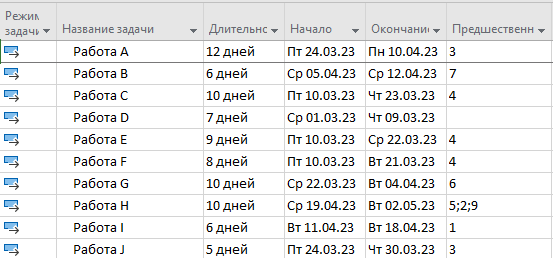
\includegraphics[scale=1.0]{imgs/task_0_0.png}
	\end{center}
	\caption{Решение тренировочного задания}
	\label{img:label}
\end{figure}

\begin{figure}[H]
	\begin{center}
		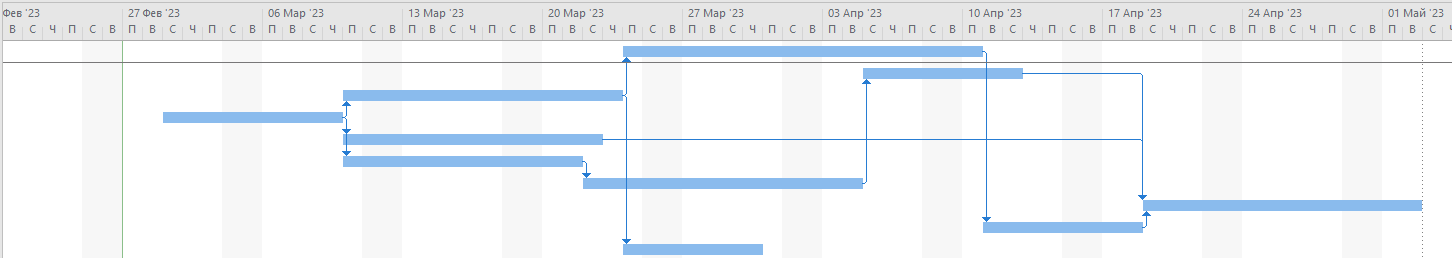
\includegraphics[width=\textwidth]{imgs/task_0_1.png}
	\end{center}
	\caption{Решение тренировочного задания (диаграмма Ганта)}
	\label{img:label}
\end{figure}
	
	\chapter{Лабораторная работа}

\section{Цель работы}

Целью лабораторной работы №1 является освоение возможностей программы Microsoft Project для планирования проекта по разработке программного обеспечения.

\section{Содержание проекта}

Команда разработчиков из 16 человек занимается созданием карты города на основе собственного модуля отображения. Проект должен быть завершен в течение 6 месяцев. Бюджет проекта: 50 000 рублей.

\section{Настройка рабочей среды проекта}

На вкладке \texttt{Проект -> Сведения о проекте} внесены параметры по условию.

\begin{figure}[H]
	\begin{center}
		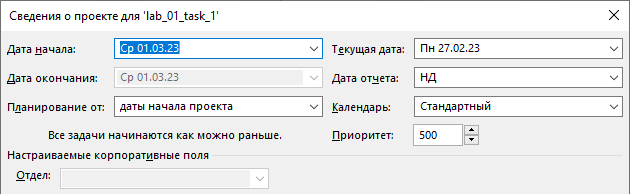
\includegraphics[scale=0.8]{imgs/task_1_0.png}
	\end{center}
	\caption{Настройка сведений о проекте}
	\label{img:label}
\end{figure}

На вкладке \texttt{Файл -> Параметры -> Расписание} установлены параметры рабочей недели и планирования.

\begin{figure}[H]
	\begin{center}
		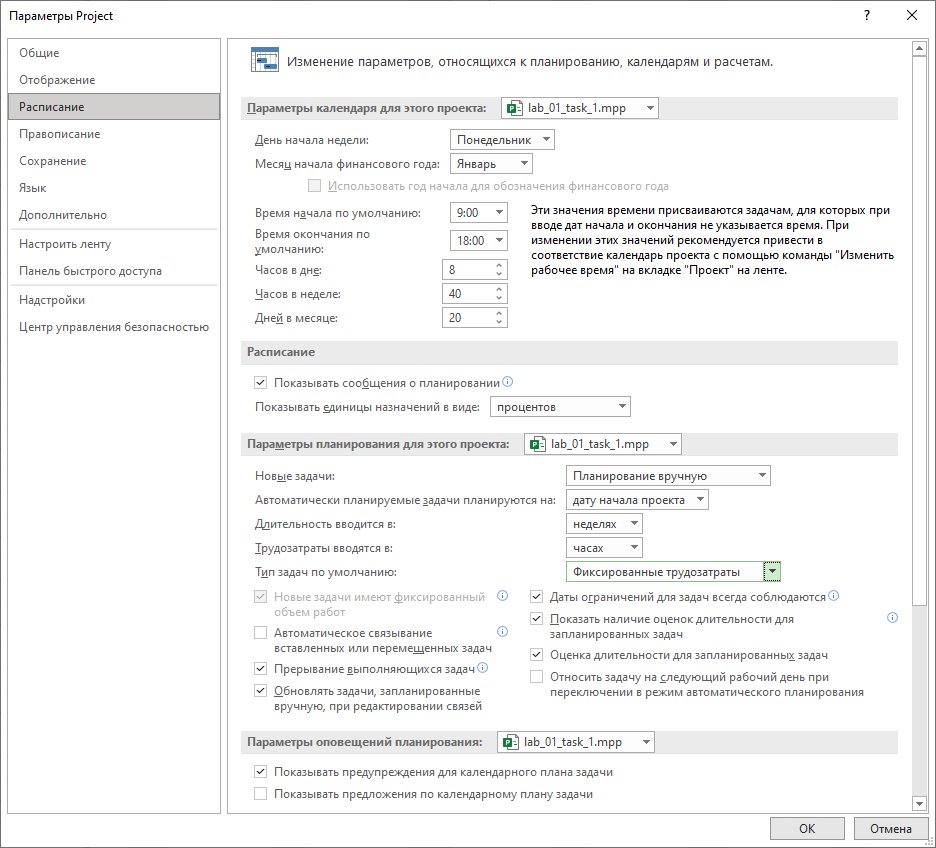
\includegraphics[width=\textwidth]{imgs/task_1_1.png}
	\end{center}
	\caption{Настройка расписания}
	\label{img:label}
\end{figure}

На вкладке \texttt{Проект -> Изменить рабочее время} установлены нерабочие праздничные дни.

\begin{figure}[H]
	\begin{center}
		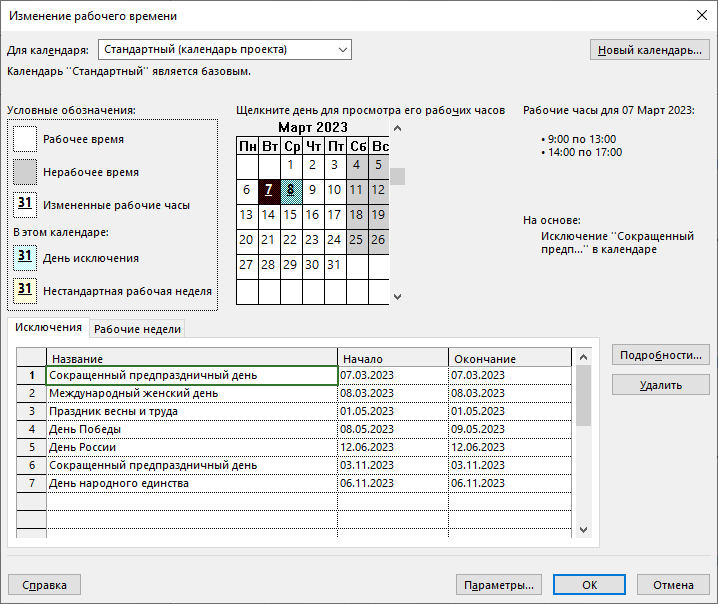
\includegraphics[width=\textwidth]{imgs/task_1_2.png}
	\end{center}
	\caption{Настройка нерабочих праздничных дней}
	\label{img:label}
\end{figure}

На вкладке \texttt{Задача -> Суммарная задача} установлена суммарная задача проекта и добавлена заметка с основной информацией о проекте.

\begin{figure}[H]
	\begin{center}
		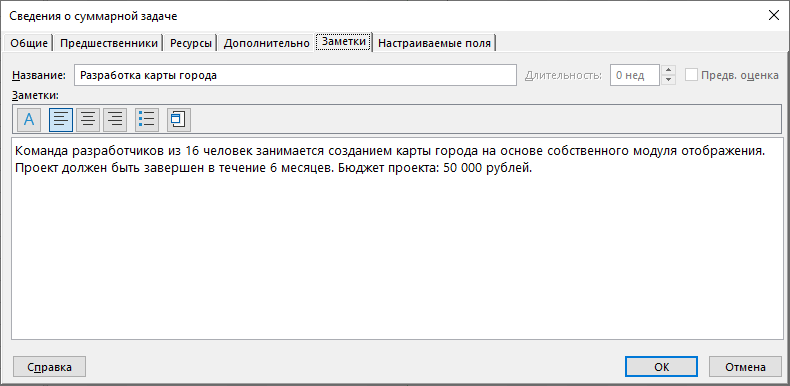
\includegraphics[width=\textwidth]{imgs/task_1_3.png}
	\end{center}
	\caption{Настройка суммарной задачи}
	\label{img:label}
\end{figure}

\section{Создание списка задач}

Осуществлен ввод задач с ручным планированием.

\begin{figure}[H]
	\begin{center}
		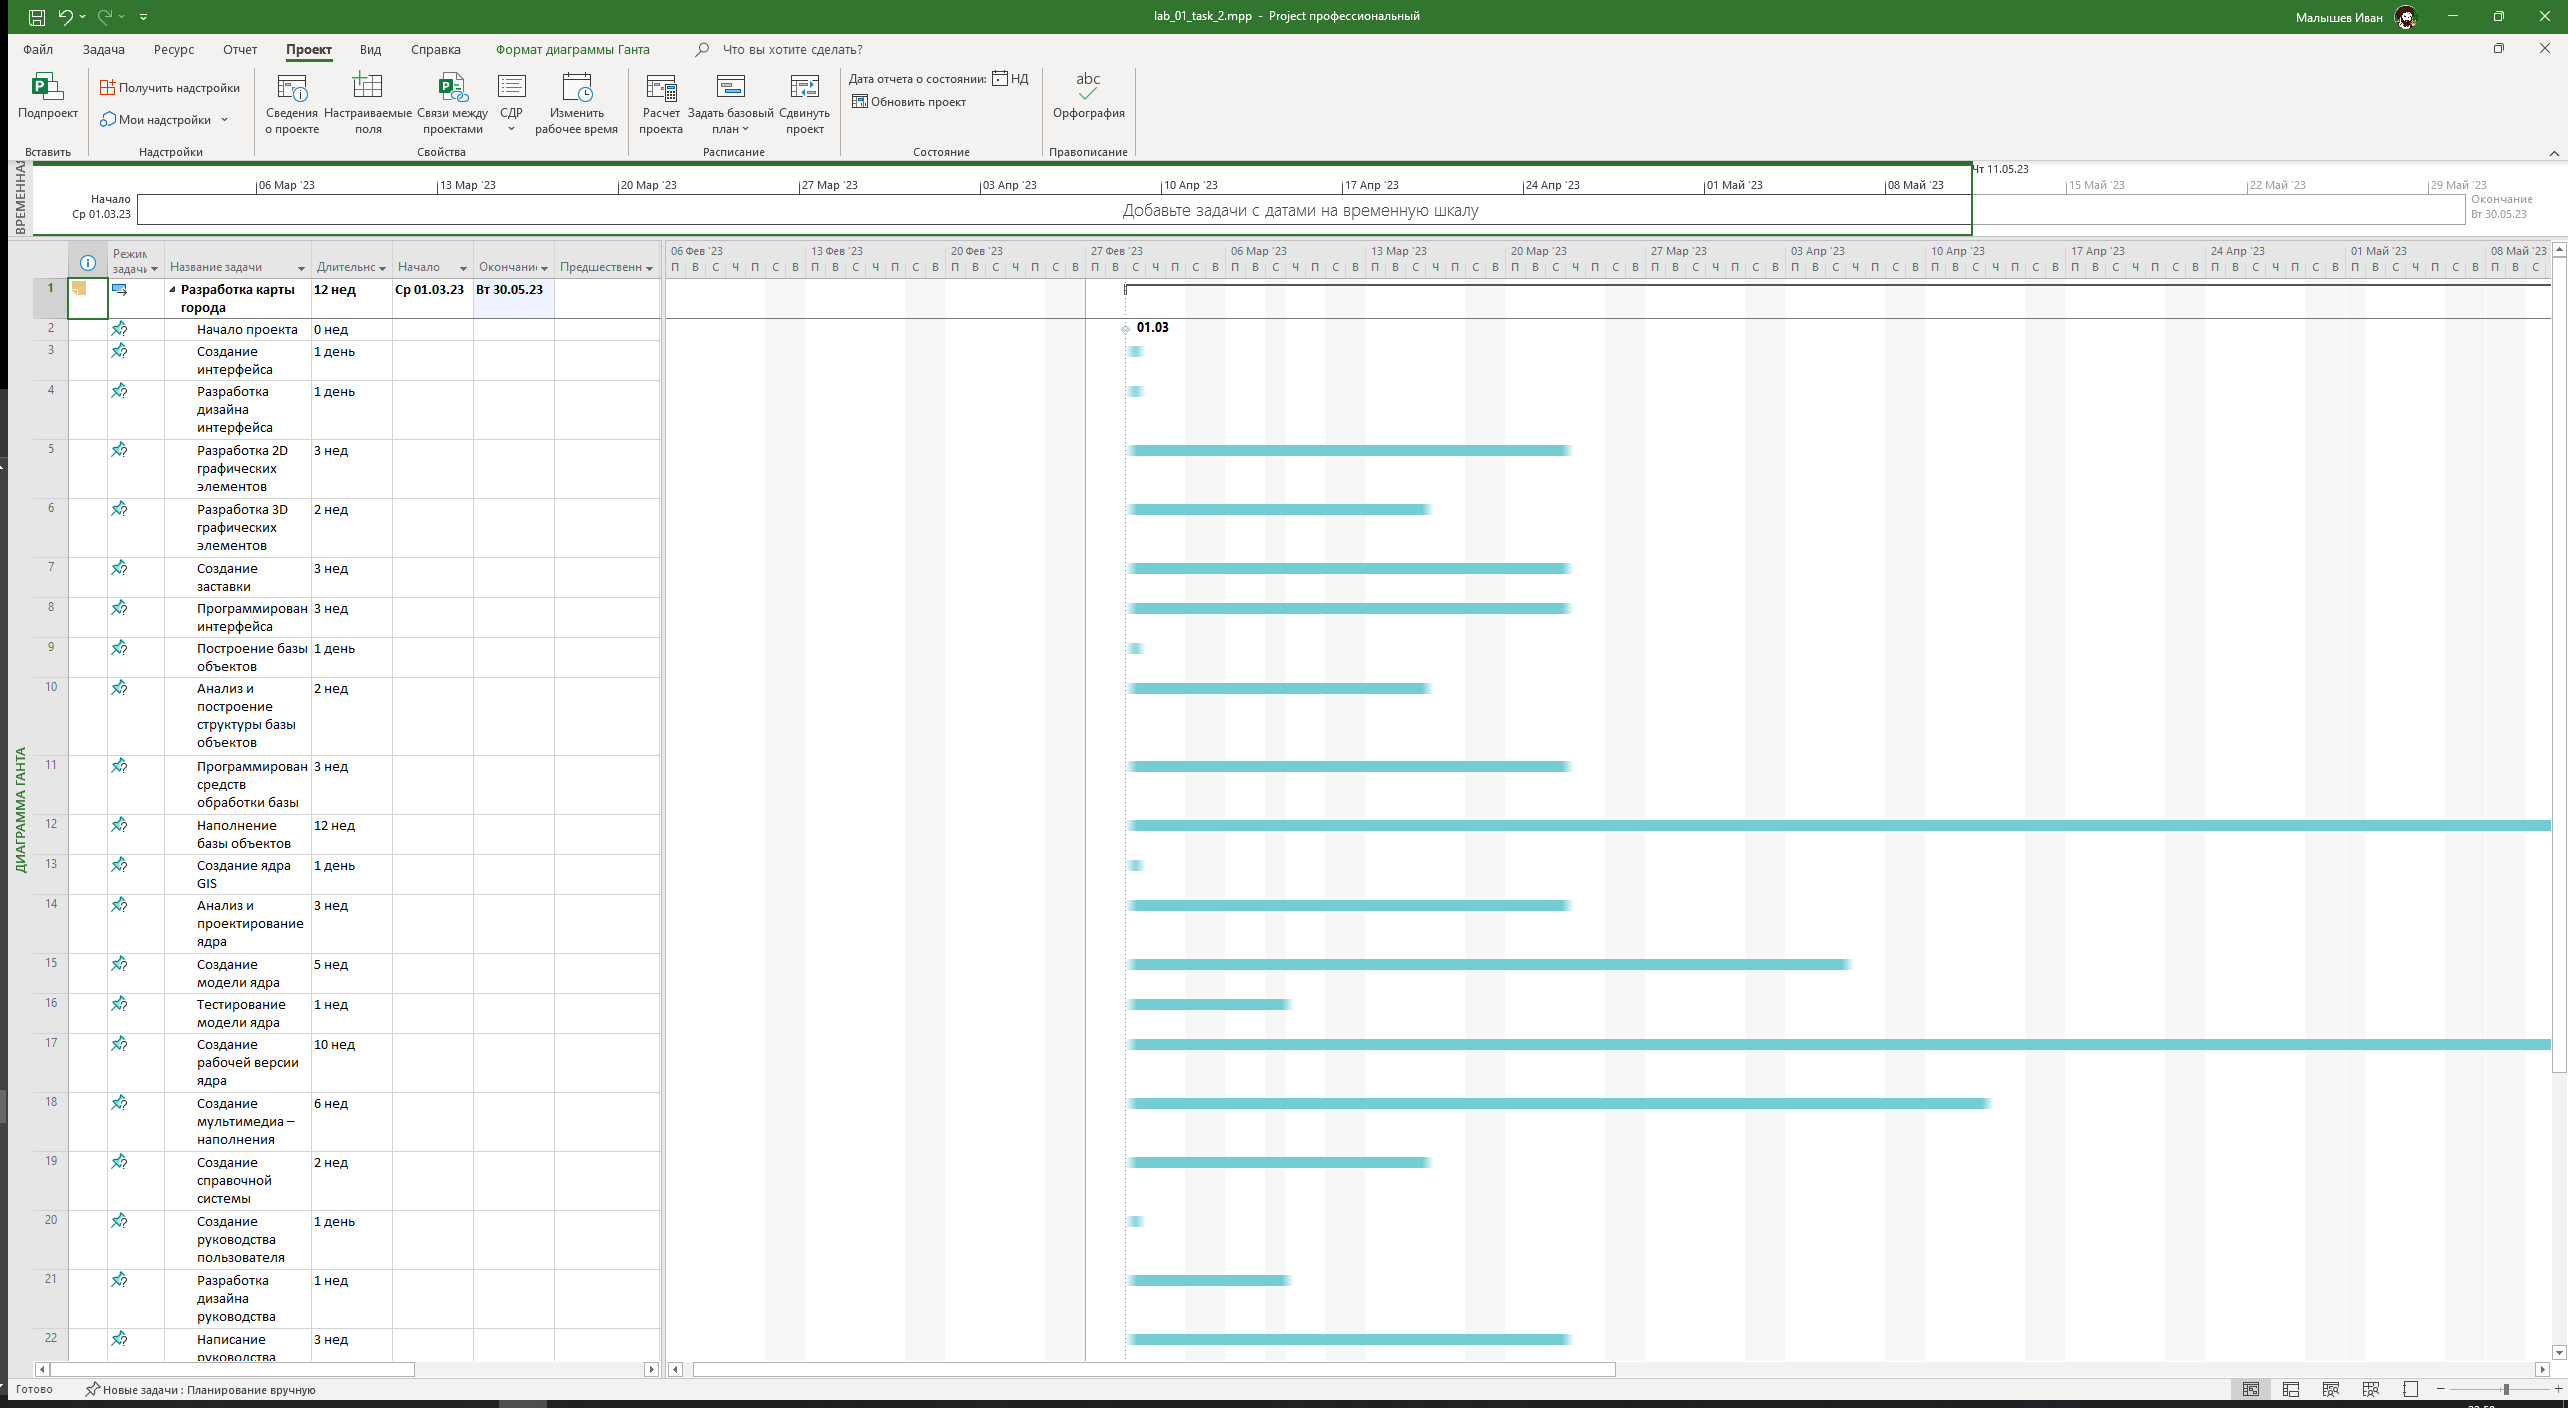
\includegraphics[width=\textwidth]{imgs/task_2_0.png}
	\end{center}
	\caption{Ввод задач}
	\label{img:label}
\end{figure}

\section{Структурирование списка задач}

При помощи кнопки \texttt{Понизить уровень задачи} были выделены подзадачи в соответствии с условием.

\begin{figure}[H]
	\begin{center}
		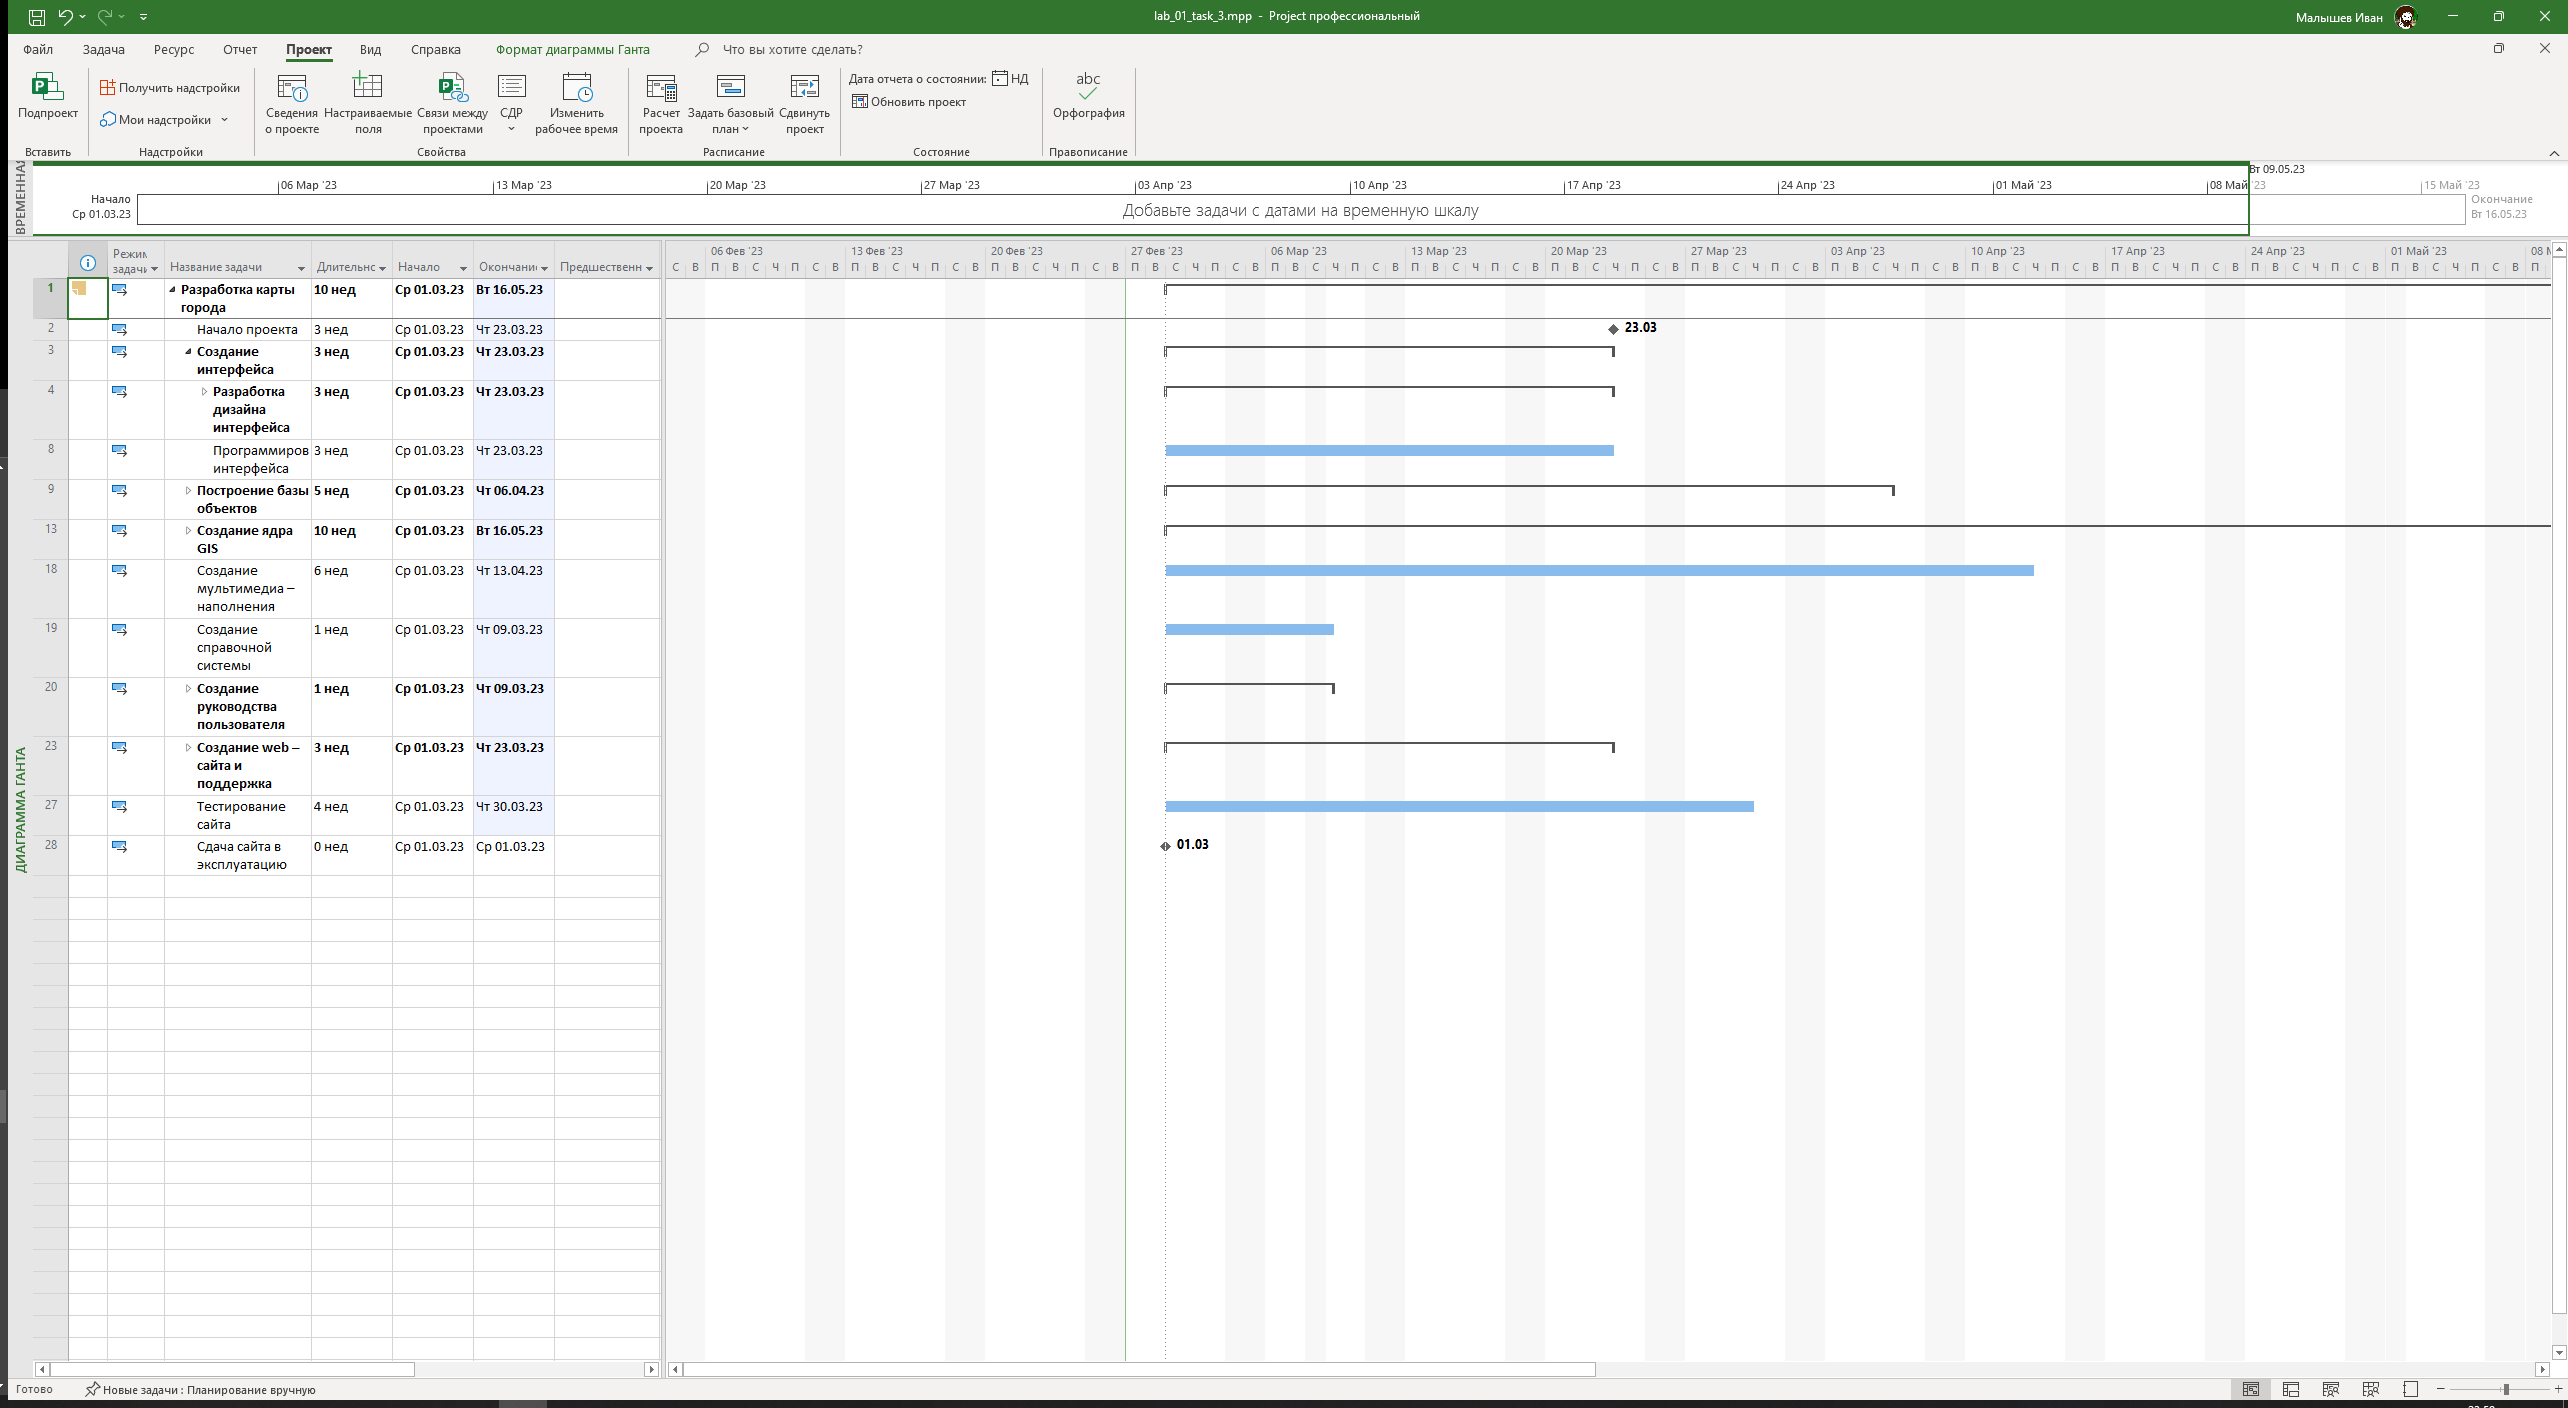
\includegraphics[width=\textwidth]{imgs/task_3_0.png}
	\end{center}
	\caption{Разбиение на подзадачи}
	\label{img:label}
\end{figure}

Также был установлен автоматический режим задач.

\section{Установление связей между задачами}

При помощи заполнения колонки \texttt{Предшественник} у каждой задачи были установлены связи между задачами.

\begin{figure}[H]
	\begin{center}
		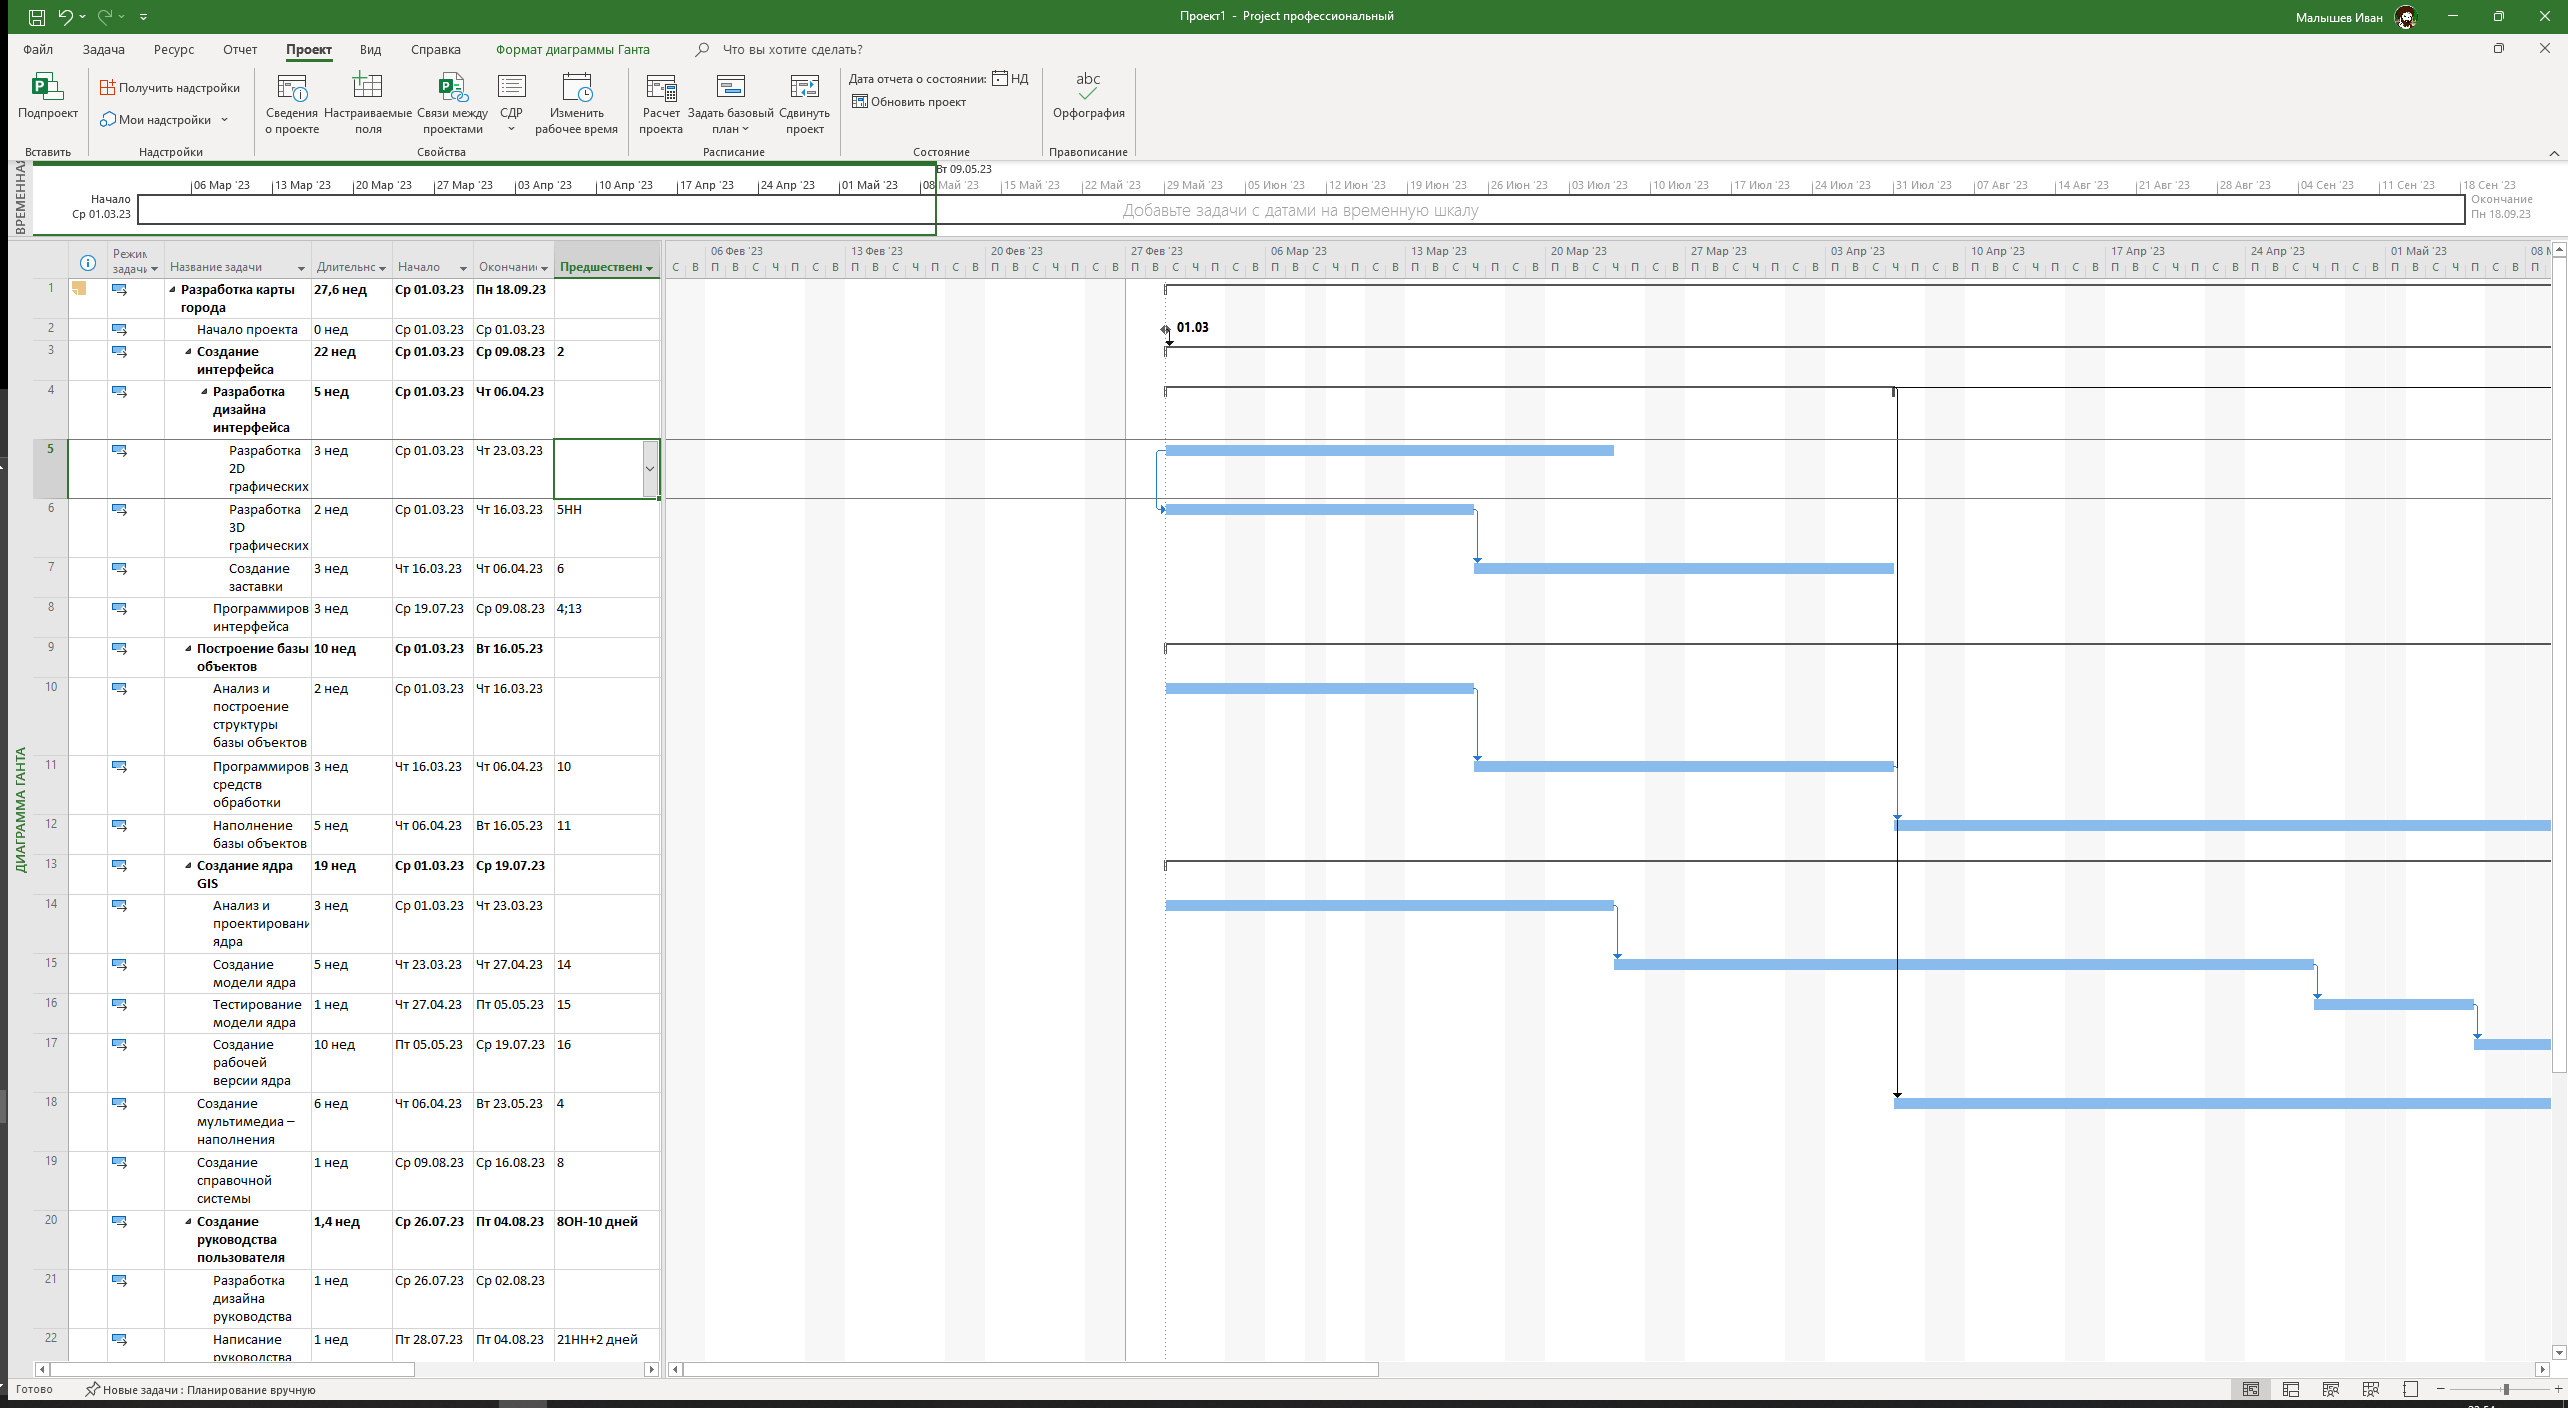
\includegraphics[width=\textwidth]{imgs/task_4_0.png}
	\end{center}
	\caption{Установленные связи между задачами}
	\label{img:label}
\end{figure}
	
	\chapter{Выводы}

В ходе выполнения данной лабораторной работы была изучена программа MS Project 2019 и ряд ее возможностей. Была проведена настройка рабочей среды, создание списка задач, их структурирование и установление связей между ними.

При установленных сроках в 6 месяцев, проект будет завершен более чем за 6 месяцев, закончившись 18 сентября 2023 года.
	
\end{document}